\documentclass{article}
\usepackage{amsmath}
\usepackage{tikz}
\usetikzlibrary{shapes.geometric}

\begin{document}

\begin{figure}[h]
    \centering
    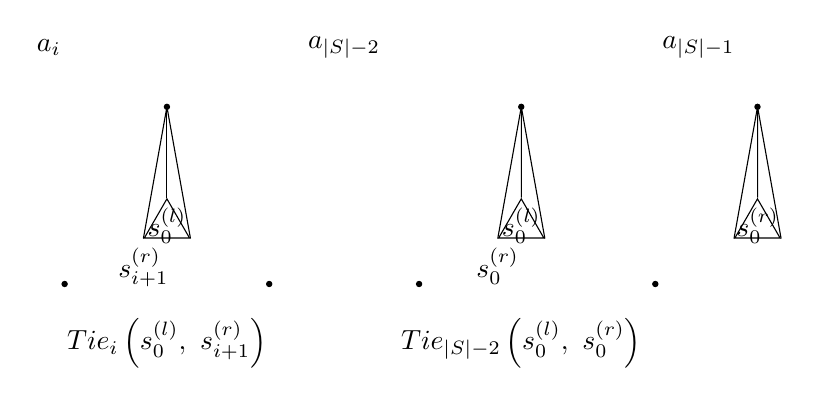
\begin{tikzpicture}[scale=1.5]
        % Left Side
        \node[regular polygon, regular polygon sides=3, draw] (tri1) at (0, 0) {};
        \node[circle, draw, fill, scale=0.2] (root1) at (0, 1) {};
        \node[circle, draw, fill, scale=0.2] (leftnode1) at (-0.866, -0.5) {};
        \node[circle, draw, fill, scale=0.2] (rightnode1) at (0.866, -0.5) {};
        
        \draw (root1) -- (tri1.corner 1);
        \draw (root1) -- (tri1.corner 2);
        \draw (root1) -- (tri1.corner 3);
        
        \node[below] at (tri1.corner 1) {$s_0^{(l)}$};
        \node[below] at (tri1.corner 2) {$s_{i+1}^{(r)}$};
        
        \node at (-1, 1.5) {$a_i$};
        
        % Right Side
        \node[regular polygon, regular polygon sides=3, draw] (tri2) at (3, 0) {};
        \node[regular polygon, regular polygon sides=3, draw] (tri3) at (5, 0) {};
        \node[circle, draw, fill, scale=0.2] (root2) at (3, 1) {};
        \node[circle, draw, fill, scale=0.2] (root3) at (5, 1) {};
        \node[circle, draw, fill, scale=0.2] (leftnode2) at (2.135, -0.5) {};
        \node[circle, draw, fill, scale=0.2] (rightnode2) at (4.135, -0.5) {};
        
        \draw (root2) -- (tri2.corner 1);
        \draw (root2) -- (tri2.corner 2);
        \draw (root2) -- (tri2.corner 3);
        
        \draw (root3) -- (tri3.corner 1);
        \draw (root3) -- (tri3.corner 2);
        \draw (root3) -- (tri3.corner 3);
        
        \node[below] at (tri2.corner 1) {$s_0^{(l)}$};
        \node[below] at (tri2.corner 2) {$s_0^{(r)}$};
        \node[below] at (tri3.corner 1) {$s_0^{(r)}$};
        
        \node at (1.5, 1.5) {$a_{|S|-2}$};
        \node at (4.5, 1.5) {$a_{|S|-1}$};
        
        \node at (0, -1) {$Tie_i\left(s_0^{(l)},\ s_{i+1}^{(r)}\right)$};
        \node at (3, -1) {$Tie_{|S|-2}\left(s_0^{(l)},\ s_0^{(r)}\right)$};
    \end{tikzpicture}
\end{figure}

\end{document}